\documentclass[oneside]{book}

\usepackage{ctex}
\usepackage{graphicx}
\usepackage{geometry}
\usepackage[hidelinks]{hyperref}
\usepackage{listings}
\usepackage{xcolor}
\usepackage{listings}
\hypersetup{
  colorlinks,
  citecolor=violet,
  linkcolor=gray,
  urlcolor=blue}
\geometry{a4paper,scale=0.8}

\title{华东师范大学算法分析助教简易手册}
\author{\href{mailto:zhzhwz@foxmail.com}{zhzhwz@foxmail.com}}

\begin{document}

\frontmatter

\maketitle

\chapter{前言}

\noindent \textbf{简介}

本手册为华东师范大学算法分析课程的助教编写,包含助教工作中可能涉及的各项流程和注意事项。

\bigbreak

\noindent \textbf{章节介绍}

第 \ref{chap:eoj} 章介绍了 EOJ 的使用方法,着重介绍了 EOJ Polygon 的使用。读者应先阅读前两节,按需阅读第 \ref{sec:polygon_operating_procedures} 节。

第 \ref{chap:elearning} 章介绍了大夏学堂的使用方法。该章暂时仅有少量工作建议,无具体操作流程。

第 \ref{chap:workflow} 章介绍了一些常见的工作流程,读者可在需要完成相应工作时参阅。

第 \ref{chap:create_problem} 章介绍了如何从零开始编写一道题。该部分属于进阶内容,请按需查阅。

\bigbreak

\noindent \textbf{更多}

欢迎在本文的\href{https://github.com/zhzhwz/ECNUAlgorithmTAManual}{仓库}提交 issue 或 PR,促进本文的完善。

若遇到无法解决的问题,可在本文的\href{https://github.com/zhzhwz/ECNUAlgorithmTAManual}{仓库}提交 issue 或直接\href{mailto:zhzhwz@foxmail.com}{邮件联系作者}。 

\bigbreak

\noindent \textbf{温馨提示}

助教工作中,请和老师保持充分的沟通。

\tableofcontents

\mainmatter

\chapter{EOJ}

\label{chap:eoj}

\section{EOJ 基础}

\label{sec:eoj_basics}

\href{https://acm.ecnu.edu.cn/}{ECNU Online Judge (EOJ)} 是由华东师范大学老师和同学维护的在线评测系统。其主要为校内师生服务,但通常可以在校外访问。目前,EOJ 主要用于托管课程上机作业和考试、各类比赛等。\footnote{由于 EOJ 题目质量参差不齐且缺乏整理,不建议在没有指导的情况下利用 EOJ 练习上机能力。对此类需求,可以移步 \href{https://www.luogu.com.cn/}{洛谷}(偏算法竞赛,有分专题题单)、\href{https://leetcode.cn/}{力扣}(偏找工作机试)等网站。}

EOJ 主要包含三部分:比赛、题目集和作业。

题目集中可以看到所有公开的题目。每个题目(无论是否公开)都有一个唯一的 ID,可以在题目集的 \# 列、题目页面的标题前、题目页面的浏览器标签、题目页面的 URL 等各处找到。在稍后取得 Polygon 使用权限后,可以直接将公开的题目被加入你管理的比赛或作业集中,但不建议这么做,详见第 \ref{ssec:copy_exist_problem} 节。

比赛与作业集类似,都包含一些题目和一个榜单。不同点在于,比赛通常只有数小时的开放时长,而作业通常有数月。大部分的比赛或作业集都是不公开的,需要权限或邀请码才能进入。在``权限''栏为绿色的勾说明该比赛或作业集是公开的,可以任意查看。比赛或作业集中的题目可能是公开的,也有可能是私有的。对于私有的题目,若你有该比赛或作业集的管理权限,则可以通过复制该题目的方法将其加入自己的比赛或作业集,详见第 \ref{ssec:copy_exist_problem} 节。

\section{EOJ Polygon 基础}

EOJ Polygon 是 EOJ 的『题目与比赛管理子系统』,可以在该系统创建并管理题目、比赛等。

\subsection{如何获取 EOJ Polygon 权限}

\label{ssec:eoj_polygon_permission}

为了创建或修改作业集,需要首先获取 EOJ Polygon 的使用权限。普通用户没有使用 EOJ Polygon 的权限,你需要联系 EOJ 的管理员以获取权限。以下是可能的寻找 EOJ 管理员的方式:

\begin{itemize}
    \item 在 EOJ 主页上寻找管理团队的联系方式(目前为 \href{mailto:acmsupport@admin.ecnu.edu.cn}{acmsupport@admin.ecnu.edu.cn}),联系时表明你的身份和需求(即,需要 EOJ Polygon 的权限),提供你的 EOJ 用户名。(推荐)
    \item 找你的课程老师,让他帮你联系算法竞赛团队的老师要权限。
    \item 加入 EOJ QQ 群(当前群号:691713742)询问。(不推荐)
\end{itemize}

\subsection{使用 EOJ Polygon}

在获取 Polygon 的权限后,你就可以在用户名的下拉菜单(如图 \ref{fig:polygon_entry_user})或者 EOJ 主页的最下方(如图 \ref{fig:polygon_entry_main_page})找到 Polygon 的入口了。EOJ 的主要创建人张羽戈在知乎写了一篇(并没有那么)详尽的文档,包含了几乎所有的 Polygon 的常见用法。详见:\href{https://zhuanlan.zhihu.com/p/59869879}{EOJ Polygon 使用指北 - 知乎}。

\begin{figure}[htbp]
  \centering
  \begin{minipage}{0.28\textwidth}
    \centering
    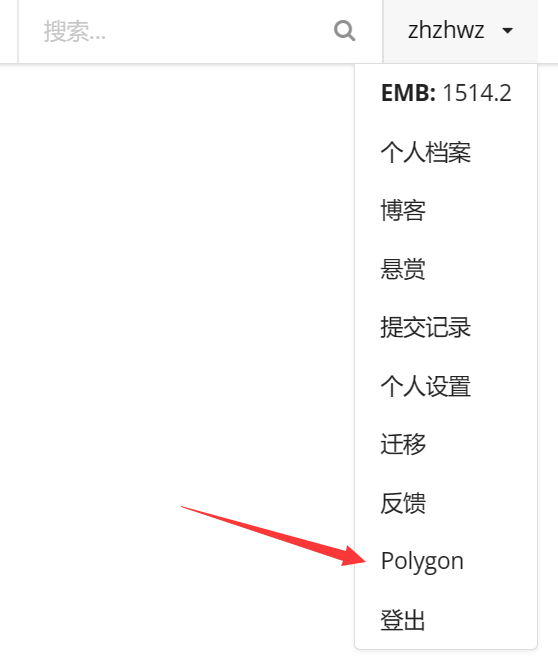
\includegraphics[width=\textwidth]{res/polygon_entry_user.png}
    \caption{用户名下拉菜单处 Polygon 入口}
    \label{fig:polygon_entry_user}
  \end{minipage}
  \begin{minipage}{0.7\textwidth}
    \centering
    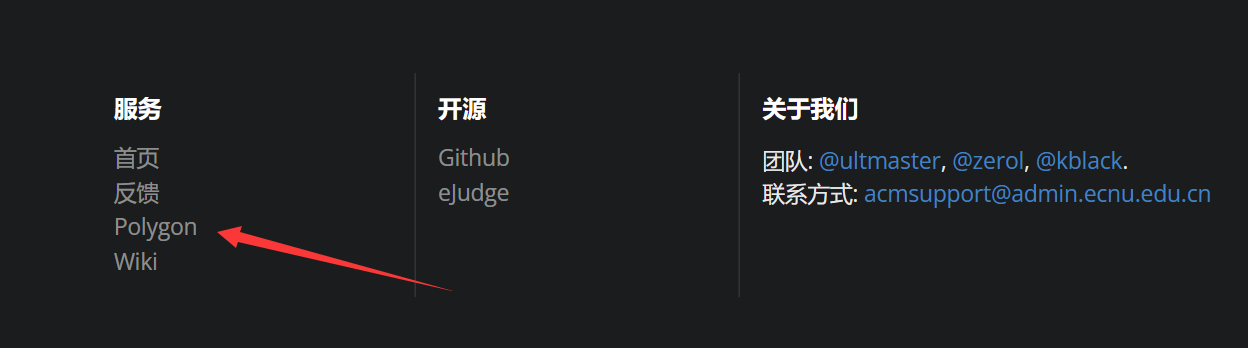
\includegraphics[width=\textwidth]{res/polygon_entry_main_page.png}
    \caption{EOJ 主页最下方处 Polygon 入口}
    \label{fig:polygon_entry_main_page}
  \end{minipage}
\end{figure}

\section{EOJ Polygon 相关常用操作流程}

\label{sec:polygon_operating_procedures}

\subsection{获取往届算法分析作业题和小测题的使用权限}

\label{ssec:permission_get}

以下是可能的方法:

\begin{itemize}
    \item 找你的课程老师,让他给你权限。前提是你的老师拥有对应作业集或比赛的权限。具体的操作步骤为:进入Polygon -- 比赛管理 -- 找到对应的作业集或比赛 -- 进入 -- 修改管理权限 -- 输入并选择要授予权限的用户 -- 点击``必须在这里保存''。
    \item 找作者要权限。前提是作者有权限。
    \item 如果想要其他作业集的权限,联系对应作业集或比赛的管理员,或直接联系 EOJ 的管理员(联系方法参见第 \ref{ssec:eoj_polygon_permission} 小节)。
\end{itemize}

\textbf{\textcolor{red}{注意:请务必在你创建的比赛或作业集中,在管理权限中加上你的老师。否则以后的助教就只能来找你要权限了。(你也可以在管理权限中加上作者(EOJ 用户名:zhzhwz))}}

\subsection{创建一个比赛或作业集}

\label{ssec:create_contest}

在 Polygon 的比赛管理中,点击 Add Contest。如有需要,也可以点击一旁的按钮复制以前的作业集作为新学期的作业集。在比赛中,有许多设置可以更改,细节请参阅\href{https://zhuanlan.zhihu.com/p/59869879}{EOJ Polygon 使用指北 - 知乎}。这里列出几项比较重要的设置:

\begin{itemize}
  \item 修改管理权限:为了使你的老师能够管理比赛或作业集,请在此处输入你老师的 EOJ ID,并点击下方的``必须在这里保存''。注意,该按钮和页面最下方的确定按钮是互斥的,点击任何一个按钮都会使其他未提交的修改失效。因此,请在修改管理权限后立刻保存;修改其他信息后先点击页面最下方的保存,再修改管理权限。
  \item 标题:对外显示的标题。可参考往届的标题。
  \item Allowed lang:一般作业可以不作修改,比赛根据实际情况删去不允许使用的语言(一般也不用改,最多删个Text)。
  \item Contest type:这项决定了这是比赛还是作业集。
  \item 开始时间、结束时间等:对于作业集,一般设置为学期初到学期末;对于比赛,则设置为比赛的起止时间。
  \item 访问控制:在完成所有其他步骤,准备开放给学生时,将其改为``仅受邀用户可见,赛后题目不公开''。
  \item 计分规则:主要使用前两种。OI 赛制有部分分,无罚时,榜单按总分排名;ACM 赛制无部分分,有罚时,榜单按通过题数第一关键字,罚时第二关键字排序。
  \item Case public:这项决定了学生在提交代码后,(无论是否通过)能否看到测试数据。对于作业,若学生提出请求,可以在和老师讨论后,设置为``评测报告总是开放''。
\end{itemize}

\subsection{导入学生名单}

\label{ssec:import_student_list}

在比赛或作业集中切换到``邀请码''页面。点击``从名单导入''。将名单经过处理后,复制到此处。系统会为每行生成一个邀请码,并将该行的内容作为该邀请码对应用户的备注。常见的备注格式如:

\begin{tabular}{lll}
10995102400 & 张三 & 1
\end{tabular}

其中最后一项为组号(若有)。复制到此处的内容应该形如:

\begin{tabular}{lll}
10995102400 & 张三 & 1 \\
10995102401 & 李四 & 1 \\
10995102402 & 王五 & 2 \\
 & $\dots$ & 
\end{tabular}

一种方便的方法是,在 Excel 中整理好名单,第一列为学号,第二列为姓名,第三列为组号。框选这三列的所有信息,复制后在导入名单处粘贴,如图 \ref{fig:excel}。系统会自动在每行的不同信息间加入制表符,最后在系统中会被转换为空格。你也可以选择其他方式处理名单后并粘贴到此处。

\begin{figure}[htbp]
  \centering
  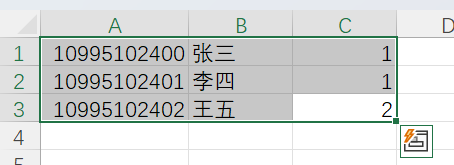
\includegraphics[width=.5\textwidth]{res/excel.png}
  \caption{框选 Excel 中的名单}
  \label{fig:excel}
\end{figure}

\subsection{导出邀请码}

\label{ssec:export_inviting_code}

在比赛或作业集的``邀请码''页面点击``导出为 csv'',将会下载一份 csv 文档,里面包含了邀请码和对应的备注。将其直接发送给学生或转换成 PDF 后发送给学生(方便在微信等不同软件中直接打开,记得检查有无出现字符重叠或部分字符未显示的情况)即可。

\subsection{复制现有的题目}

\label{ssec:copy_exist_problem}

可以复制的题目主要包括两种类型:EOJ 题目集中公开的题目和你管理的或作业集中的题目。此外,也可以复制你管理的题目,但一般没有必要。

复制题目后,相当于创建了原题的一个副本,你对其有完全的管理权限,可以任意修改它的题面、数据、时限等。与此同时,原题的任何修改将不会影响到副本,也没有办法方便地将原题的修改同步到副本上。

对于 EOJ 题目集中公开的题目,尽管可以直接将它们添加到比赛或作业集中,仍然建议首先复制题目,并把副本加入比赛或作业集。这么做可以保证你有对该题目的修改权限,以应对之后可能出现的各种情况。在 Polygon 的题目管理中,点击 Request Clone,输入题目的 ID(在第 \ref{sec:eoj_basics} 节有介绍)即可。

对于你管理的比赛或作业集中的题目,你可能没有题目本身的权限。在 Polygon 的题目管理中,点击 Request Clone,根据提示输入 \lstinline{<ContestID>-<ProblemID>}。其中,\lstinline{<ContestID>} 可以在比赛或作业集页面的 URL 中找到,\lstinline{<ProblemID>} 指的是题目在该比赛或作业集中的 ID,即比赛或作业集页面``题目''页面中 \# 一栏。

\subsection{创建题目}

\label{ssec:create_new_problem}

通常不会用到这个功能。然而,如果你需要自己原创题目或将其他网站的题目搬运到 EOJ,则需要创建题目。在题目管理中,点击``Add Problem'',输入一个仅由英文和数字构成的题目别名。这个名字不是很重要,可以随便取。之后,就会跳转到题目的管理页面。

在发布之前,有一些工作要完成:

\begin{itemize}
  \item 添加管理员:一般可以省去这一步骤。然而,如果你希望别人也有管理该题目的权限,请在概览的基本信息处点击编辑,在管理员列表中输入他们的 ID 并选择,之后点击 OK。
  \item 添加题面:题面会展示给做题者。在``题面''页面中,点击 Add Statement。在各个框内填入内容,支持 Markdown 语法。完成后,点击页面最下方的确定。之后,可以预览题面的展示效果。如需修改,在``题面''页面中,点击对应题面最右方的 Edit。如需预览,则点击对应题面 Name 一栏的超链接。如果创建了多个题面,请将要展示的题面设置为 Active。
  \item 添加数据。题目需要测试点才能评测。可以手填数据,但通常会上传一个压缩包,包含输入输出的数据。压缩包内的文件需要满足一定的格式才能被识别。一般,文件名可以标为 \lstinline|1.in|, \lstinline|1.out|, \lstinline|2.in|, \lstinline|2.out|, $\dots$, \lstinline|10.in|, \lstinline|10.out|,即每组数据两个文件,其中 in 为输入,out 为对应的输出,系统会自动识别文件名。一些其他的文件名,例如将 \lstinline|.out| 换成 \lstinline|.ans|、\lstinline|.o| 等通常也都可以识别。若压缩包较大,可能需要等待一段时间才能上传完毕。之后,可以单独设置每组数据。勾选加入样例则做题者可以在题面看见这组数据,包括输入和输出;勾选是有效的测试点后这组数据才会被评测。通常会把样例取消勾选是有效的测试点或者将分数设置为0分。
  \item 编辑时限和内存限制:一般可以使用默认的配置。但如果你的题目有特殊需求,可以在概览中编辑。
\end{itemize}

完成所有的工作后,在概览页面点击发布。

\subsection{将题目添加到比赛或作业集}

\label{ssec:add_problem_to_contest}

在比赛或作业集的``题目''页面,在最上方的 Search for problems 中输入题目 ID,选择后点击 Add。只有公开题目或你管理的题目才能被搜索到并添加到比赛或作业集。如果希望添加其他题目,例如不由你管理的比赛或作业集中的私有题目,请联系该比赛或作业集的管理员或者 EOJ 的管理员以获取授权。

你可以上下拖动题目以更改其排列顺序。需要点击 Save orders 以保存。

\subsection{更新题目}

\label{ssec:update_problem}

在题目管理中,点击要更新的题目后的 Latest Version。对于已经发布的题目,右上角有一个``只读版本''的提示。需要点击其中的复制,创建新版本后才能修改。常见的需要修改的部分可以参见第 \ref{ssec:create_new_problem} 小节。修改完成后,点击概览页面的发布。之后,可以在``已发布的版本''查看效果。

\subsection{重判题目}

\label{ssec:rejudge_problem}

在更改了题目的时限、数据等内容后,可能需要重判已有的提交。提交有两种类型,一种是直接在题目下的提交,提交的页面 URL 一般为 \lstinline|https://acm.ecnu.edu.cn/problem/<problem ID>/|;另一种是在比赛或作业集中的提交,题目被加入比赛或作业集后,通过该比赛或作业集访问的都属于这种提交。其页面 URL 一般为 \lstinline|https://acm.ecnu.edu.cn/contest/<contest ID>/problem/<problem ID in contest>/|。

对于前一种提交,需要在题目的管理界面,切换到``提交''页面。该页面可以看到所有提交,包括通过比赛或作业集进行的提交。点击某一提交对应的重判即可重判该提交,无论它是通过何种途径提交的。点击最上方的重判可以重判所有\textbf{\color{red} 直接在题目下进行的提交},在比赛或作业集中的提交将不会被重判。

对于后一种提交,在比赛或作业集的管理界面,切换到``提交''页面,可以看到所有该比赛或作业集中的提交。若需要重判某一特定提交,点击提交最后的重判即可,也可以参考上一段的方法在题目的管理页面重判。若需要重判某一题的所有提交或该比赛或作业集的所有提交,点击最上方的重判。可以选择重判某题或所有题。

\subsection{下载榜单}

\label{ssec:download_ranking_list}

在比赛结束后可能需要下载榜单以统计成绩。在比赛或作业集的前台,选择榜单,将鼠标移至``重新计算''右侧的齿轮,选择``下载为 csv''。

\chapter{大夏学堂}

\label{chap:elearning}

% TODO: add details

由于作者目前已无法登录大夏学堂,此处只能给出一些工作建议。欢迎补充该部分文档。

\section{工作建议}

\subsection{作业批改}

\begin{enumerate}
  \item 大夏学堂的作业批改功能存在许多问题,例如文件加载慢、批注框对中文支持很差(容易出现空格)等问题。建议的解决方案:将作业下载到本地分类,批改完后再将分数和批改意见依次填回。
  \item 批改时记录一下每次作业的易错点或常见问题,方便之后作业讲评时使用。
\end{enumerate}


\chapter{常见工作流程}

\label{chap:workflow}

\section{工作前的准备}

\begin{enumerate}
  \item 若没有 EOJ 账号,创建一个。
  \item 熟悉 EOJ 的基本功能。
  \item 参考第 \ref{ssec:permission_get} 小节的方法获取 EOJ Polygon 的权限。
  \item 参考第 \ref{sec:polygon_operating_procedures} 节熟悉 EOJ Polygon。简单熟悉即可,后续可以根据具体需要查阅其中相关章节。
\end{enumerate}

\section{创建作业集}

\begin{enumerate}
  \item 参考第 \ref{ssec:create_contest} 小节的方法创建作业集。
  \item 参考第 \ref{ssec:import_student_list} 小节的方法导入学生名单。
  \item 参考第 \ref{ssec:export_inviting_code} 小节的方法导出邀请码,发送给学生。
  \item 参考第 \ref{sec:set_homework} 节布置第一次作业。
\end{enumerate}

\section{布置一次作业}

\label{sec:set_homework}

\begin{enumerate}
  \item 和老师沟通,确定本次作业的题数和每题的主题或涉及算法。
  \item 寻找相关题目。以下是可能的方法:
  \begin{itemize}
    \item 在之前的作业集中选择合适的题目。若无对应作业集权限,参考第 \ref{ssec:permission_get} 小节的方法获得之前作业集的权限。
    \item 在 EOJ 公开题目中寻找相关题目。
    \item 在其他 OJ 获取题面和数据。作者已知目前唯一能够方便获取数据的 OJ 仅有 \href{https://loj.ac/}{LOJ} ,但其题目难度普遍偏高,请谨慎挑选。
    \item 在其他 OJ 获得题面,并自己造数据。包括但不限于\href{https://www.luogu.com.cn/}{洛谷}等 OJ 的题面可以直接在题目界面复制 markdown 源代码。造数据的方法可以参见第 \ref{sec:generating_data} 节。
    \item 从零开始自行创建题目。见第 \ref{chap:create_problem} 章。
  \end{itemize}
  \item 和老师沟通选定的题目是否合适。
  \item 对于 EOJ 已有所需题目的情况,复制现有的题目,见第 \ref{ssec:copy_exist_problem} 小节;否则,在准备好材料后创建题目,见第 \ref{ssec:create_new_problem} 小节。
  \item 将题目添加到作业集,见第 \ref{ssec:add_problem_to_contest} 小节。
\end{enumerate}

\section{准备一次小测}

\begin{enumerate}
  \item 和老师沟通,确定小测的题量、算法、难度、是否需要原创题等信息。
  \item 参照第 \ref{ssec:create_contest} 小节创建一个比赛。
  \item 寻找相关题目。具体方法参见第 \ref{sec:set_homework} 节。需要注意的是,小测题目对于原创性的要求会更高,请尽量保证每位参与的同学都没有做过原题。(考虑到小测的目的是检测同学们的学习成果,题目与作业中的题目有相似性是允许的。)
  \item 和老师沟通选定的题目是否合适。
  \item 对于 EOJ 已有所需题目的情况,复制现有的题目(由于原创性需要,尽量不要使用 EOJ 已有的题目),见第 \ref{ssec:copy_exist_problem} 小节;否则,在准备好材料后创建题目,见第 \ref{ssec:create_new_problem} 小节。
  \item 将题目添加到比赛,见第 \ref{ssec:add_problem_to_contest} 小节。
  \item 若包含原创题,建议参考第 \ref{sec:verify_problem} 节邀请同学验题。
\end{enumerate}

\section{题目出现问题,需要修改}

\begin{enumerate}
  \item 参考第 \ref{ssec:update_problem} 小节更正题目。
  \item 参考第 \ref{ssec:rejudge_problem} 小节重判已有的提交。
\end{enumerate}

\section{导出上机作业或小测成绩}

参考第 \ref{ssec:download_ranking_list} 小节在对应比赛或作业集下载榜单。

\chapter{从零开始创建一道题}

\label{chap:create_problem}

本章的内容对于无算法竞赛基础的读者可能难度较大。考虑到实际工作中可能会用到,此处给出一些简单的指引。若读完仍感觉无从下手,请咨询身边的朋友(如,有算法竞赛经历或出题经历的同学等)。

除了本文外,你也可以参考一些网络上的资料,如\href{https://oi-wiki.org/contest/problemsetting/}{出题 - OI-Wiki}等。

\section{构思}

在进行所有工作前,需要先对题目进行构思。通常题目的灵感来自于某个算法、某个游戏、某个生活中的小问题等。

在构思阶段需要完成对题目的基本设计,包括题目大意、大致的输入输出格式、标准解答、根据标答设计的数据范围,此外还有可能的其他相对简单的解答与其对应的数据范围、各个数据范围对应的分值。

确保题目考查的算法没有超纲,难度适宜。对一次比赛,还需要综合考虑各题的难度,需要简单题和较难题,题目一般在比赛中按难度升序排列。

\section{编写题面}

有两种出题风格。一种是根据题目大意设计一个背景,用讲故事的方法描述问题;另一种是直接用术语描述问题本身。两种方法均可,但要确保以下几点:

\begin{itemize}
  \item 在关键的部分语言表达精确,避免产生歧义。例如,在图论相关问题中,表达清楚是有向图还是无向图。
  \item 格式规范。公式和数字应用 Markdown 格式,写在两个 \$ 符号之间。中文和英文或数字之间应用一个空格隔开,英文或数字和标点之间不用隔开。
  \item 写清输入输出的格式。应有至少一组样例,在 EOJ Polygon 添加样例的方法参见第 \ref{ssec:create_contest} 小节。
  \item 在提示中写清数据范围。若有多个不同的数据范围,写清各自的分数占比。
\end{itemize}

\section{编写标程}

当前应该已经确定题目描述和输入输出的格式。编写标程并尽量确保其正确性,常见的方法如手算样例与标程对比,另写一份更能保证正确性的暴力代码并\href{https://oi-wiki.org/contest/common-tricks/}{对拍}等。

如题目包含部分分,还应编写部分分对应的代码。稍后利用该代码测试部分分,见第 
\ref{sec:test_partial_score} 节。

如果题目为交互题或多解题,可能还需要编写交互器或检查器。请参考 \href{https://oi-wiki.org/tools/testlib/}{Testlib - OI Wiki} 以了解如何编写。参考 \href{https://zhuanlan.zhihu.com/p/59869879}{EOJ Polygon 使用指北 - 知乎} 以了解如何将其部署到题目。

\section{造数据}

\label{sec:generating_data}

题目的数据量通常很大,因此需要利用程序生成测试数据。通常可以另外编写一个程序生成输入数据,输出到文件。可以在程序中只生成一份数据,用命令行参数来控制数据规模,并用脚本多次调用以生成所有数据,也可以一次性生成所有数据。此外,也可以考虑用 Testlib 的 \href{https://oi-wiki.org/tools/testlib/generator/}{Generator - OI Wiki} 生成输入数据。

之后,通过编写脚本,多次调用标程,将输入重定向到输入文件,输出重定向到输出文件,即可完成数据的生成。

\section{测试部分分}

\label{sec:test_partial_score}

完成上述步骤后,先参考第 \ref{ssec:create_new_problem} 小节发布一个版本。之后,将之前编写的各个部分分的代码提交到 EOJ,看得到的分数是否与预期相同。若不同,检查是否存在问题,调整数据范围、题目时限等。

\section{验题}

\label{sec:verify_problem}

完成上述所有工作后,一道题基本已经创建完毕了。然而,人难免有失误,题目描述是否清晰、标程是否有误、难度是否适中仍无法确定。找几个你比较熟悉他们水平的朋友,邀请他们来做题,以更好地评估这些内容,并根据反馈再做调整。

通常,可以开一个作业集,将访问控制设置为仅比赛管理员可见,将所有验题人全部设为这一作业集的管理员,他们就能够在 EOJ 的``作业''页面找到这一作业集,并访问其中题目,具体流程参考第 \ref{ssec:create_contest} 小节。该作业集应只用于验题,正式比赛应另开作业集。

\end{document}
